\documentclass[journal,12pt,twocolumn]{IEEEtran}

\usepackage{setspace}
\usepackage{gensymb}

\singlespacing


\usepackage[cmex10]{amsmath}

\usepackage{amsthm}

\usepackage{mathrsfs}
\usepackage{txfonts}
\usepackage{stfloats}
\usepackage{bm}
\usepackage{cite}
\usepackage{cases}
\usepackage{subfig}

\usepackage{longtable}
\usepackage{multirow}

\usepackage{enumitem}
\usepackage{mathtools}
\usepackage{steinmetz}
\usepackage{tikz}
\usepackage{circuitikz}
\usepackage{verbatim}
\usepackage{tfrupee}
\usepackage[breaklinks=true]{hyperref}
\usepackage{graphicx}
\usepackage{tkz-euclide}

\usetikzlibrary{calc,math}
\usepackage{listings}
    \usepackage{color}                                            %%
    \usepackage{array}                                            %%
    \usepackage{longtable}                                        %%
    \usepackage{calc}                                             %%
    \usepackage{multirow}                                         %%
    \usepackage{hhline}                                           %%
    \usepackage{ifthen}                                           %%
    \usepackage{lscape}     
\usepackage{multicol}
\usepackage{chngcntr}

\DeclareMathOperator*{\Res}{Res}

\renewcommand\thesection{\arabic{section}}
\renewcommand\thesubsection{\thesection.\arabic{subsection}}
\renewcommand\thesubsubsection{\thesubsection.\arabic{subsubsection}}

\renewcommand\thesectiondis{\arabic{section}}
\renewcommand\thesubsectiondis{\thesectiondis.\arabic{subsection}}
\renewcommand\thesubsubsectiondis{\thesubsectiondis.\arabic{subsubsection}}


\hyphenation{op-tical net-works semi-conduc-tor}
\def\inputGnumericTable{}                                 %%

\lstset{
%language=C,
frame=single, 
breaklines=true,
columns=fullflexible
}
\begin{document}


\newtheorem{theorem}{Theorem}[section]
\newtheorem{problem}{Problem}
\newtheorem{proposition}{Proposition}[section]
\newtheorem{lemma}{Lemma}[section]
\newtheorem{corollary}[theorem]{Corollary}
\newtheorem{example}{Example}[section]
\newtheorem{definition}[problem]{Definition}

\newcommand{\BEQA}{\begin{eqnarray}}
\newcommand{\EEQA}{\end{eqnarray}}
\newcommand{\define}{\stackrel{\triangle}{=}}
\bibliographystyle{IEEEtran}
\providecommand{\mbf}{\mathbf}
\providecommand{\pr}[1]{\ensuremath{\Pr\left(#1\right)}}
\providecommand{\qfunc}[1]{\ensuremath{Q\left(#1\right)}}
\providecommand{\sbrak}[1]{\ensuremath{{}\left[#1\right]}}
\providecommand{\lsbrak}[1]{\ensuremath{{}\left[#1\right.}}
\providecommand{\rsbrak}[1]{\ensuremath{{}\left.#1\right]}}
\providecommand{\brak}[1]{\ensuremath{\left(#1\right)}}
\providecommand{\lbrak}[1]{\ensuremath{\left(#1\right.}}
\providecommand{\rbrak}[1]{\ensuremath{\left.#1\right)}}
\providecommand{\cbrak}[1]{\ensuremath{\left\{#1\right\}}}
\providecommand{\lcbrak}[1]{\ensuremath{\left\{#1\right.}}
\providecommand{\rcbrak}[1]{\ensuremath{\left.#1\right\}}}
\theoremstyle{remark}
\newtheorem{rem}{Remark}
\newcommand{\sgn}{\mathop{\mathrm{sgn}}}
\providecommand{\abs}[1]{\vert#1\vert}
\providecommand{\res}[1]{\Res\displaylimits_{#1}} 
\providecommand{\norm}[1]{\Vert#1\rVert}
%\providecommand{\norm}[1]{\lVert#1\rVert}
\providecommand{\mtx}[1]{\mathbf{#1}}
\providecommand{\mean}[1]{E[ #1 ]}
\providecommand{\fourier}{\overset{\mathcal{F}}{ \rightleftharpoons}}
%\providecommand{\hilbert}{\overset{\mathcal{H}}{ \rightleftharpoons}}
\providecommand{\system}{\overset{\mathcal{H}}{ \longleftrightarrow}}
	%\newcommand{\solution}[2]{\textbf{Solution:}{#1}}
\newcommand{\solution}{\noindent \textbf{Solution: }}
\newcommand{\cosec}{\,\text{cosec}\,}
\providecommand{\dec}[2]{\ensuremath{\overset{#1}{\underset{#2}{\gtrless}}}}
\newcommand{\myvec}[1]{\ensuremath{\begin{pmatrix}#1\end{pmatrix}}}
\newcommand{\mydet}[1]{\ensuremath{\begin{vmatrix}#1\end{vmatrix}}}
\numberwithin{equation}{subsection}
\makeatletter
\@addtoreset{figure}{problem}
\makeatother
\let\StandardTheFigure\thefigure
\let\vec\mathbf
\renewcommand{\thefigure}{\theproblem}
\def\putbox#1#2#3{\makebox[0in][l]{\makebox[#1][l]{}\raisebox{\baselineskip}[0in][0in]{\raisebox{#2}[0in][0in]{#3}}}}
     \def\rightbox#1{\makebox[0in][r]{#1}}
     \def\centbox#1{\makebox[0in]{#1}}
     \def\topbox#1{\raisebox{-\baselineskip}[0in][0in]{#1}}
     \def\midbox#1{\raisebox{-0.5\baselineskip}[0in][0in]{#1}}
\vspace{3cm}
\title{Assignment-2}
\author{Satya Sangram Mishra}
\maketitle
\newpage
\bigskip
\renewcommand{\thefigure}{\theenumi}
\renewcommand{\thetable}{\theenumi}
Download all python codes from 
\begin{lstlisting}
https://github.com/satyasm45/Summer-Internship/tree/main/Assignment-2/Codes
\end{lstlisting}
%
and latex-tikz codes from 
%
\begin{lstlisting}
https://github.com/satyasm45/Summer-Internship/tree/main/Assignment-2
\end{lstlisting}
%
\section{Question No. 2.28}
Construct a quadrilateral ABCD such that AB =5, \angle A =50$^\circ$
, AC = 4, BD = 5 and AD = 6.
%
\section{Explanation}
For this quadrilateral adjacent side lengths AB,AD and diagonal BD is known. So,points A,B and D can be pin-pointed from it.Assuming we are restricted to first quadrant we have:
\begin{align}
\vec{A} = \myvec{0\\0}, \vec{B} = \myvec{5\\0}, \vec{D} = \myvec{p\\q}
\end{align}
Then,
\begin{align}
\norm{\vec{B}-\vec{A}} = \norm{\vec{B}}  = 5  \quad \brak{\because \vec{A}=0}
\end{align}
\begin{align}
\norm{\vec{D}-\vec{A}}^2 = \norm{\vec{D}}^2  = p^2+q^2  \quad \brak{\because \vec{A}=0}
\end{align}
\begin{align}
\norm{\vec{D}-\vec{B}}^2 = \norm{\myvec{p\\q}-\myvec{5\\0}}^2  = (p-5)^2+q^2  
\end{align}

Also AD=6 and BD=5, So
\begin{align}
\norm{\vec{D}-\vec{A}}^2 &= p^2+q^2=36
\end{align}
\begin{align}
\norm{\vec{D}-\vec{B}}^2 &= (p-5)^2+q^2=25
\end{align}
Solving for p and q from above equations and considering values in first 
quadrant we have:
\begin{align}
p=3.6;q=4.8
\end{align}
We still have to find co-ordinates of C. The only information we are left
with is AC=4 and \angle A =50$^\circ$.
But we can note that \angle A =50$^\circ$ does not give us any additional
information than what we already have. Once A,B and D are fixed, angle of A
is also fixed. 

So we have to verify that whether this value matches
with the given value.
  
We have,
A=Angle between BA and DA. 

So, cos A= $$\frac{(\textbf{B}-\textbf{A})^T.(\textbf{D}-\textbf{A})}{\norm{\vec{B}-\vec{A}}\norm{\vec{D}-\vec{A}}}$$
\implies cos A=$(\textbf{B}^T.\textbf{D})/(\norm{\vec{B}}\norm{\vec{D}})$
\quad \brak{\because \vec{A}=0}
 $$\implies cos A=(5*3.6+4.8*0)/(5*6)=0.6$$
 $$\implies \angle A=arccos(0.6)$$
 
 So \angle{A}=53.13$^\circ$.
 
 
 But \angle{A}=50$^\circ$\ is given which causes a mismatch. Therefore construction of quadrilateral with given measurements is not possible.


\numberwithin{figure}{section}
\begin{figure}[!ht]
\centering
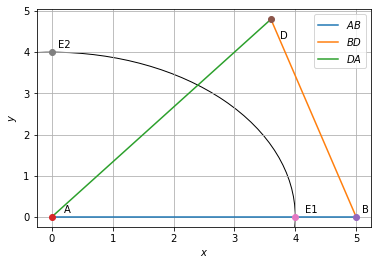
\includegraphics[width=\columnwidth]{figure2}
\caption{ Partial Construction}
\label{fig:right_angle_triangle}	
\end{figure}


Additionally,From the above figure we can also argue that after drawing an ARC taking A as center and radius 4 many feasible values for C are possible.But no feasible C can alter $\angle {A}$ and change it to 50$^\circ$.
So,No quadrilateral is possible.

\end{document}